\documentclass[a4paper]{paper}

\usepackage[utf8]{inputenc}
\usepackage{amsmath}
\usepackage[left=2.5cm,top=3cm,right=2.5cm,bottom=3cm,bindingoffset=0.cm]{geometry}
\usepackage{bm} % used for bold math symbols
\usepackage{parskip} % vertical space instead of indented paragraphs
\usepackage{hyperref}
\usepackage{graphicx}


\DeclareMathOperator\sign{sign}


\author{
Patrick Spieler \\
\texttt{stapelzeiger@gmail.com}
}

\title{Aircraft Dynamics}

\begin{document}
\maketitle
\hrule
\bigskip


\begin{abstract}

This document summarizes the equations of rigid body \& aircraft dynamics as well as other models used for the simulator.

\end{abstract}

\tableofcontents

\pagebreak

\section{Rigid Body Dynamics}

All the dynamic equations are written in the body frame.

Euler's equation for rigid body dynamics (from F. Landis Markley, John L. Crassidis - Fundamentals of Spacecraft Attitude Determination and Control p.84):

\begin{equation}
    \dot{\bm\omega}_{Ib}^b = {I^b_{CM}}^{-1} \left(\bm\tau^b_{CM} - \bm\omega_{Ib}^b \times (I^b_{CM} \bm\omega_{Ib}^b)\right)
\end{equation}

To transform the inertia tensor $I^b_{CM}$ from the aircraft frame $a$ to the body frame $b$, use:

\begin{equation}
    I^b_{CM} = R_a^b I^a_{CM} {R_a^b}^T
\end{equation}

\section{Aerodynamic Forces}

Aerodynamic forces are a function of airspeed $V_a$. Airspeed is the velocity vector of the aircraft with respect to the surrounding air. Airspeed is related to ground speed $V_g$ (velocity of the aircraft with respect to ground) and wind speed $V_w$ (velocity of the wind with respect to ground) by the following vector equality:

\begin{equation}
    \bm{V}_g = \bm{V}_a + \bm{V}_w
\end{equation}

\subsection{Airplane}

For a plane, the direction of the airspeed with respect to the body frame is expressed with two angles $\alpha$ and $\beta$, called angle of attack and angle of side-slip respectively.
The positive direction of these angles are as shown in figure \ref{fig:alpha_beta}:

\begin{figure}[h]
\centering
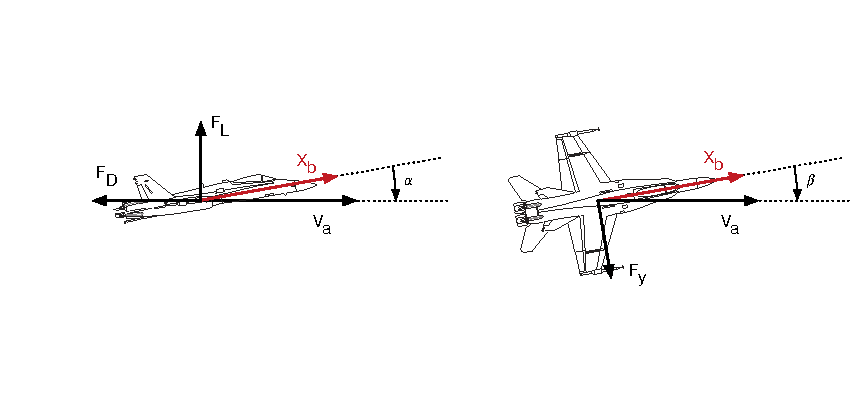
\includegraphics[width=\textwidth]{img/alpha_beta.pdf}
\caption{positive $\alpha$ and $\beta$, base image source: F-18 HARV from Dryden Flight Research Center Graphics Collection: https://www.dfrc.nasa.gov/Gallery/Graphics/index.html}
\label{fig:alpha_beta}
\end{figure}

The airspeed vector expressed in the body frame as a function of $\alpha$ and $\beta$ is given by (Mark Drela - Flight Vehicle Aerodynamics, chapter 9.5):

\begin{equation}
    \bm{V}_a^b = V_a  \left(\begin{matrix} \cos\alpha \cos\beta\\
    \sin{\beta}\\
    \sin\alpha \cos\beta\end{matrix}\right)
\end{equation}

\begin{equation}
\begin{split}
    V_a &= \lVert \bm{V}_a^b \lVert\\
    \alpha &= \arctan\left(\frac{V_a^b_z}{V_a^b_x}\right)\\
    \beta &= \arctan\left(\frac{V_a^b_y}{\sqrt{(V_a^b_x)^2 + (V_a^b_z)^2}}\right)
\end{split}
\end{equation}

From the above formula it follows that to obtain the attitude of the plane with respect to the airflow the plane is first rotated around $\bm{z}_b$ by $-\beta$ and then rotated around $\bm{y}_b'$ by $\alpha$.


\subsubsection{Forces and Moments}

Aerodynamic forces of a plane are decomposed as lift $\bm F_L$, drag $\bm F_D$ and side force $\bm F_y$. The direction of the lift and drag forces in the body frame changes with angle of attack, whereas the side force is always along the y body axis as shown in figure \ref{fig:alpha_beta}.

The total aerodynamic force on an airplane is given by:
\begin{equation}
    \bm F_{aero}^b = \bm F^b_L + \bm F^b_D + \bm F^b_y = \left(\begin{matrix}
        - \cos\alpha F_D + \sin\alpha F_L\\
        F_y\\
        - \sin\alpha F_D - \cos\alpha F_L
    \end{matrix}\right)
\end{equation}

The aerodynamic moments around $\bm x_b$, $\bm y_b$ and $\bm z_b$ are called $\bm l$, $\bm m$ and $\bm n$ respectively.
\begin{equation}
    \bm \tau_{aero}^b = \left(\begin{matrix}
    l\\ m \\ n
    \end{matrix}\right)
\end{equation}

\subsubsection{Control Surfaces}

\begin{itemize}
    \item $\delta_a$ Aileron, positive to roll right (left aileron down, right aileron up)
    \item $\delta_e$ Elevator, positive to pitch up
    \item $\delta_r$ Rudder, positive to yaw right
\end{itemize}

The unit of the control surface deflections is radian.

\subsubsection{Aerodynamic Coefficients}

The forces above can be obtained from aerodynamic coefficients using (Randal Beard, Timothy McLain - Small Unmanned Aircraft Theory and Practice):
\begin{equation}
\begin{split}
    F_L &= \frac{1}{2} \rho V_a^2 S C_L(\alpha, q, \delta_e) \\
    F_D &= \frac{1}{2} \rho V_a^2 S C_D(\alpha, q, \delta_e) \\
    m &= \frac{1}{2} \rho V_a^2 S c C_m(\alpha, q, \delta_e) \\
    F_y &= \frac{1}{2} \rho V_a^2 S C_Y(\beta, p, r, \delta_a, \delta_r) \\
    l &= \frac{1}{2} \rho V_a^2 S b C_l(\beta, p, r, \delta_a, \delta_r) \\
    n &= \frac{1}{2} \rho V_a^2 S b C_n(\beta, p, r, \delta_a, \delta_r) \\
\end{split}
\end{equation}

where:
\begin{itemize}
    \item $S$: wing area
    \item $c$: mean aerodynamic cord
    \item $b$: wing span
\end{itemize}
and the angular rates of the aircraft with respect to the air in the body frame are:
\begin{equation}
    \bm \omega_{aero}^b = \left(\begin{matrix}
    p\\ q \\ r
    \end{matrix}\right)
\end{equation}

\subsubsection{Linearized Model}

The linear model is obtained from a first order Taylor expansion of the coefficients as a function of control surfaces, flow angle and rate.

\begin{equation}
\begin{split}
    C_L(\alpha, q, \delta_e) &\approx C_{L_0} + C_{L_\alpha}\alpha + C_{L_q} \frac{c}{2V_a} q + C_{L_{\delta_e}}\delta_e \\
    C_D(\alpha, q, \delta_e) &\approx C_{D_0} + C_{D_\alpha}\alpha + C_{D_q} \frac{c}{2V_a} q + C_{D_{\delta_e}}\delta_e \\
    C_m(\alpha, q, \delta_e) &\approx C_{m_0} + C_{m_\alpha}\alpha + C_{m_q} \frac{c}{2V_a} q + C_{m_{\delta_e}} \delta_e \\
    C_Y(\beta, p, r, \delta_a, \delta_r) &\approx C_{Y_0} + C_{Y_\beta} \beta + C_{Y_p} \frac{b}{2V_a}p + C_{Y_r} \frac{b}{2V_a}r + C_{Y_{\delta_a}}\delta_a + C_{Y_{\delta_r}}\delta_r \\
    C_l(\beta, p, r, \delta_a, \delta_r) &\approx C_{l_0} + C_{l_\beta} \beta + C_{l_p} \frac{b}{2V_a}p + C_{l_r} \frac{b}{2V_a}r + C_{l_{\delta_a}}\delta_a + C_{l_{\delta_r}}\delta_r \\
    C_n(\beta, p, r, \delta_a, \delta_r) &\approx C_{n_0} + C_{n_\beta} \beta + C_{n_p} \frac{b}{2V_a}p + C_{n_r} \frac{b}{2V_a}r + C_{n_{\delta_a}}\delta_a + C_{n_{\delta_r}}\delta_r \\
\end{split}
\end{equation}

This model can be improved by adding nonlinear stall behavior to the lift and drag coefficients (Randal Beard, Timothy McLain - Small Unmanned Aircraft Theory and Practice).

\begin{equation}
\begin{split}
    C_L(\alpha, q, \delta_e) &\approx C_L(\alpha) + C_{L_q} \frac{c}{2V_a} q + C_{L_{\delta_e}}\delta_e \\
    C_D(\alpha, q, \delta_e) &\approx C_D(\alpha) + C_{D_q} \frac{c}{2V_a} q + C_{D_{\delta_e}}\delta_e \\
\end{split}
\end{equation}

The lift is a blending of the linear relationship and the lift of a flat plate:
\begin{equation}
    C_L(\alpha) = (1-\sigma(\alpha))\left(C_{L_0} + C_{L_\alpha}\alpha\right) + \sigma(\alpha)\left( 2 \sign(\alpha)\sin^2\alpha \cos\alpha \right)
\end{equation}

where $\sigma(\alpha)$ is a sigmoid function that blends the two models.
\begin{equation}
    \sigma(\alpha) = \frac{1 + e^{-M(\alpha-\alpha_{max})} + e^{M(\alpha+\alpha_{max})}}{(1+e^{-M(\alpha-\alpha_{max})})(1 + e^{M(\alpha+\alpha_{max})})}
\end{equation}
with $M$ a positive constant that determines the transition rate and $\alpha_{max}$ the (positive) stall angle of attack.

The lift coefficient $C_{L_\alpha}$ can be obtained approximately by:
\begin{equation}
    C_{L_\alpha} = \frac{\pi AR}{1 + \sqrt{1 + (AR/2)^2}}
\end{equation}

with the aspect ratio $AR$ defined as:
\begin{equation}
    AR := b^2/S
\end{equation}

The drag coefficient is given by the sum of a parasitic drag $C_{D_p}$ and an induced drag that is proportional to the square of the lift.
\begin{equation}
    C_D(\alpha) = C_{D_p} + \frac{(C_{L_0} + C_{L_\alpha}\alpha)^2}{\pi e AR}
\end{equation}
where $e$ is the Oswald efficiency factor, which is between 0.8 and 1.0.

\section{Actuator Model}

Servo actuators are modeled as position and rate limited devices.

\section{Environment Models}

\subsection{Atmosphere}

\subsection{Wind}

constant + shear over ground

dryden turbulence tf

\subsection{Gravity}

cst

\subsection{Magnetic Field}

cubeth?

\section{Sensor Models}

gyro

acc

static pressure

dynamic pressure

mag

gps

altitude distance

\end{document}
